% Schematic representation of z-axis layout
% Modified from a version created by Henrik Kröger, 
%https://github.com/derhedwig/fiberoptics/blob/master/auswertung.tex
% Author: Orlando Torres (2016)

\documentclass{standalone}
\usepackage{amsmath} % Required for \varPsi below
\usepackage{tikz,pgfplots}
\usepackage{pst-plot}
\usetikzlibrary{calc}
\usetikzlibrary{patterns}

\begin{document}
  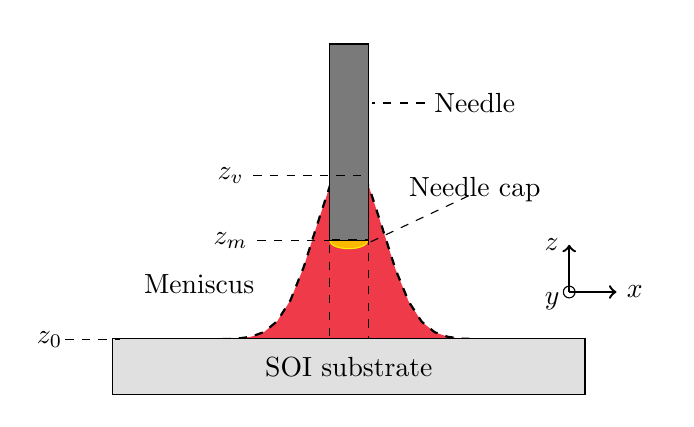
\begin{tikzpicture}[domain=0:4]
   	%define colors
    \definecolor{bbblue}{rgb}{0.262,0.709,0.613}
    \definecolor{rrred}{rgb}{0.933, 0.227, 0.286}
    \definecolor{yyyellow}{rgb}{0.933, 0.756, 0.227}
    \definecolor{gre}{rgb}{0.878, 0.878, 0.878}
    \definecolor{gre3}{rgb}{0.478, 0.478, 0.478}
    \definecolor{gre2}{rgb}{0.578, 0.778, 0.578}
    \definecolor{orange}{rgb}{0.980, 0.721, 0}
    %define coordinates for modulator (upper side)
    \coordinate (z1) at (0, 9mm);
    \coordinate (z2) at (0, -20mm);
    \coordinate (z3) at (0, -19.5mm);
    \coordinate (ax) at (28mm, -10mm);
    
    
    \draw[thick, domain=-20mm:20mm,dashed, fill=rrred] plot({\x-2.4mm},{-1.6+((2.3 * exp(-(\x/7 -1)^2/6)))}) ;    
    % Substrate, modulators, Waveguides, MMI and converters %    
    \draw [yellow,fill=orange](0,-3.5mm) ellipse (2.4mm and 1mm) ;
    \node [shape=rectangle, minimum width=80.3mm, minimum height=47mm, color=white, draw]
    (substrate) at (0mm,0mm) {};
    \node [shape=rectangle, minimum width=5mm, minimum height=25mm, 
    fill=gre3, draw] (needle) at(z1) {};
    %substrate
    \node [shape=rectangle, minimum width=60mm, minimum height=7.1mm, 
    fill=gre, draw] (surf) at(z3) {};
    \node [shape=rectangle, minimum width=5mm, minimum height=12.5mm, 
    dashed, draw] (dev2) at(0,-9.6mm) {};
    
    
 \node [shape=circle, color=black, fill=white, inner sep=1.5, draw]
    (substrate) at (ax) {};
 \draw (ax) node [text width=3mm] (axx) at + (-1.6mm,-1.2mm) {$y$};
 \draw [->, to path={-| (\tikztotarget)},line width=0.30mm, color=black, draw]  (ax) -- ($(ax) + (0,6mm)$) node[left] {$z$};
 \draw [->, to path={-| (\tikztotarget)},line width=0.30mm, color=black, draw]  (ax) -- ($(ax) + (6mm,0)$) node[right] {$x$};
\node [align=center] (subs) at (-15mm, 4.8mm) {$z_v$}; 
\draw [dashed] (subs) -- ($(subs)  + (17.6mm, 0)$);

\node [align=center] (subs) at (-15mm, -3.5mm) {$z_m$}; 
\draw [dashed] (subs) -- ($(subs)  + (17.6mm, 0)$);

\node [align=center] (subs) at (-38mm, -16mm) {$z_0$}; 
\draw [dashed] ($(subs)  - (-2mm, 0)$)-- ($(subs)  + (9mm, 0)$);

\node [align=center] (subs) at (0, -19.5mm) {SOI substrate}; 
\node [align=center] (subs) at (16mm, 14mm) {Needle};
\draw [dashed] (subs) -- ($(subs)  + (-13mm, 0)$);
\node [align=center] (subs) at (16mm, 3mm) {Needle cap}; 
\draw [dashed] ($(subs)  + (-0.8mm,-0.8mm)$) -- ($(subs)  + (-14mm, -7mm)$); 
\node [align=center] (subs) at (-19mm, -9mm) {Meniscus}; 

  \end{tikzpicture}

\end{document}